\documentclass[10pt]{scrartcl}
\usepackage{amsmath,amsthm,amssymb,mathtools,xfrac}
\usepackage{enumerate}
\usepackage[utf8]{inputenc}
%\usepackage{german}
\usepackage{a4wide}
\usepackage{graphics}
\usepackage{graphicx}
\usepackage[T1]{fontenc}
\usepackage{epsfig}
\usepackage{libertine}
\usepackage[pdftex]{hyperref}
\usepackage{refcount}
\usepackage{framed}
\usepackage{xcolor}
\usepackage{multicol}
\usepackage{enumitem}
\usepackage{caption}
\usepackage{gensymb}
\usepackage[export]{adjustbox}

\topmargin-.5in \textheight9in \oddsidemargin0in \textwidth6.5in

\begin{document}

\begin{minipage}{.5\textwidth}
{\scshape Department of Mathematics and Informatics \\
University of Cologne\\}
\small Prof. Dr. Gregor Gassner \\
\small Dr. Andrés Rueda-Ramírez \\
\end{minipage}
\hfill
\begin{minipage}{.3\textwidth}
\begin{flushright}

\includegraphics[width=3cm]{figs/logo-uni-koeln.jpg}\\
\today
\end{flushright}
\end{minipage}

\begin{center}
{\Large\bfseries
An Introduction to Climate Modeling with Julia}\\
\vspace{0.2cm}
{\bfseries Milestone 5 - Constructing a System Matrix with FD Approach}
\end{center}


\section{Constructing a System Matrix with FD Approach}

In this milestone, you will build the heart of the climate model: the system matrix for solving the energy balance model.
The EBM model reads
\begin{equation}
C(x)\frac{\partial T}{\partial t}+A(CO_2)+BT - \underbrace{\vec{\nabla} \cdot (D(x)\nabla T)}_{L} = S_\text{sol}(x,t)
\label{EBM}
\end{equation}
in spherical coordinates on the sphere's surface with the pair $ (\tilde{\theta},\varphi)$
\begin{equation}
L(\tilde{\theta},\varphi) = \csc^2(\tilde{\theta})\frac{\partial}{\partial \varphi}\left(\tilde{D} \frac{\partial T}{\partial \varphi}\right)+\frac{\partial}{\partial \tilde{\theta}}\left(\tilde{D} \frac{\partial T}{\partial \tilde{\theta}}\right)+ \cot(\tilde{\theta})\tilde{D}\frac{\partial T}{\partial \tilde{\theta}}
\label{Operator}
\end{equation}
When we apply the finite difference method, we have for each degree of freedom:
\begin{equation}
\frac{\partial T_{j,i}}{\partial t} \approx \underbrace{\frac{L_{j,i}}{C_{j,i}} - \frac{B}{C_{j,i}} T_{j,i}}_{R_{j,i}(T)} + \underbrace{ \frac{1}{C_{j,i}} \left(S_{\text{sol}, j, i}(t) - A\right)}_{F_{j,i}}
\label{DoF}
\end{equation}
The discretization of the heat conduction term on the surface of a sphere with a Cartesian mesh of cell size $h$ (uniform for latitude and longitude) reads:

\begin{itemize}
\item For the inner degrees of freedom:
\begin{equation} \label{innerDoF}
\begin{split}
L_{j,i} = \frac{\csc^2(\tilde{\theta}_{j,i})}{h^2}\Big(-2\tilde{D}_{j,i}T_{j,i}&+\left[\tilde{D}_{j,i}-\frac{1}{4}(\tilde{D}_{j,i+1}-\tilde{D}_{j,i-1})\right]T_{j,i-1}  \\
& \left. + \left[\tilde{D}_{j,i}+\frac{1}{4}(\tilde{D}_{j,i+1}-\tilde{D}_{j,i-1})\right]T_{j,i+1}\right) \\
+ \frac{1}{h^2}\Big(-2\tilde{D}_{j,i}T_{j,i}&+\left[\tilde{D}_{j,i}-\frac{1}{4}(\tilde{D}_{j+1,i}-\tilde{D}_{j-1,i})\right]T_{j-1,i}  \\
& \left. +\left[\tilde{D}_{j,i}+\frac{1}{4}(\tilde{D}_{j+1,i}-\tilde{D}_{j-1,i})\right]T_{j+1,i}\right) \\
 + \cot(\tilde{\theta}_{j,i})\frac{\tilde{D}_{j,i}}{2h}&\left[T_{j+1,i}-T_{j-1,i}\right]
\end{split}
\end{equation}

\item For the degrees of freedom at the poles:
\begin{align}
L_{1,i} &= \frac{\sin(h/2)}{4 \pi \text{area[1]}}\sum^{\text{n\_longitude}}_{k=1}\frac{1}{2}\left(\tilde{D}_{1,k}+\tilde{D}_{2,k}\right)\left[T_{2,k}-T_{1,k}\right], \\
L_{\text{n\_latitude},i} &= \frac{\sin(h/2)}{4 \pi \text{area[n\_latitude]}}\sum^{\text{n\_longitude}}_{k=1}\frac{1}{2}\left(\tilde{D}_{\text{n\_latitude},k}+\tilde{D}_{\text{n\_latitude-1},k}\right)\left[T_{\text{n\_latitude-1},k}-T_{\text{n\_latitude},k}\right]
\label{polesDoF}
\end{align}
for all $i \in \{1,\dots,\text{n\_longitude}\}$, where $\texttt{area[1]} := \texttt{area[n\_latitude]} := 0.5\left(1-\cos\left(h/2\right)\right)$ contains the normalized area of the polar cap.

\end{itemize}
\newpage
To implement the model, proceed as follows:

\begin{enumerate}
\item[1.] Implement the mesh as a struct in Julia or a class in Python with a constructor.


\begin{table}[!h]
\small
	\begin{center}
	\begin{tabular}{|c|c|}
	\hline
	\textit{Parameter}& \textit{Description} \\
	\hline
	\texttt{n\_latitude} & \text{Number of DOFs in longitude} \\
	\texttt{n\_longitude} & \text{Number of DOFs in latitude} \\
	\texttt{ndof}& \text{Total number of DOFs}  \\
	\texttt{h}& \text{Cell size in latitude direction in radians}  \\
	\texttt{geom}& \text{Geometrical parameter at poles with} $\text{geom} = \frac{\sin(h/2)}{4\pi \texttt{area[1]}}$  \\
	\texttt{csc2}& \text{Metric term for the transformation to spherical coordinates, the vector with entries $\csc^2(\tilde{\theta}_j)$}  \\
	\texttt{cot}& \text{Metric term for the transformation to spherical coordinates, the vector with entries $\cot(\tilde{\theta}_j)$}  \\
	\texttt{area}& \text{Area of each cell on the surface of the sphere which only depends on latitude}  \\
	\hline
	\end{tabular}
	\end{center}
\end{table}

\item[2.] Calculate the earth surface type dependent heat conduction coefficients $\tilde{D}(\tilde{\theta},\varphi) \in \mathbb{R}^{n_y \times n_x}$ by implementing a function \small\texttt{\detokenize{calc_diffusion_coefficients}} \normalsize that maps the following equation:

\begin{align}
\tilde{D}(\tilde{\theta},\varphi) \in \mathbb{R}^{n_y \times n_x} =
\begin{cases}
\tilde{D}_{\text{ocean},\text{poles}}+ (\tilde{D}_{\text{ocean},\text{equ}} - \tilde{D}_{\text{ocean},\text{poles}})\sin(\tilde{\theta})^5& \text{for the ocean} \\
\tilde{D}_\text{NP} + (\tilde{D}_\text{equ} - \tilde{D}_\text{NP})\sin(\tilde{\theta})^5  &  \text{for the Northern Hemisphere} \\
\tilde{D}_\text{SP} + (\tilde{D}_\text{equ} - \tilde{D}_\text{SP})\sin(\tilde{\theta})^5  & \text{for the Southern Hemisphere} \\
\end{cases}
\end{align}

\bigskip
\noindent
The corresponding thermal conductivity coefficient\footnote{K. Zhuang, G.R. North, M.J. Stevens, {\em A NetCDF version of the two-dimensional energy balance model based on the full multigrid algorithm}, SoftwareX, Vol. 6, pp. 198-202, July 7, 2017.} are as follows:

\begin{table}[!h]
\small
	\begin{center}
	\begin{tabular}{|c|c|}
	\hline
	\textit{Types}& \textit{Thermal conductivity in $W/m^2/K$} \\
	\hline
	Ocean at Poles& $ 0.4$ \\
	Ocean at Equator&  $ 0.65$ \\
	Equator& $ 0.65$ \\
	North Pole& $ 0.28$ \\
	South Pole& $ 0.2$ \\
	\hline
	\end{tabular}
\caption{Surface specific thermal conductivity for the determination of diffusion coefficients}
	\label{thermal conductivity}
	\end{center}
\end{table}

Note: For the surface type dependency of the heat conduction, you will once again need to include the function \small\texttt{\detokenize{read_geography}} \normalsize from milestone 1.


\item[3.] Use the above formulas, the function \small\texttt{\detokenize{calc_diffusion_coefficients}} \normalsize and the functions for the other parameters from previous milestones to write a function \small\texttt{\detokenize{compute_equilibrium_EBM_2D}} \normalsize to compute the EBM for two spatial dimensions using a forward Euler time integration scheme. Try to calculate the EBM using this function. What happens?

\item[4.] Write a function \small\texttt{\detokenize{calc_jacobian_ebm_2d}} \normalsize that computes the Jacobian matrix of the FD operator numerically. You can calculate the $j$-th column of the Jacobian matrix with the equation:

\begin{equation*}
\underline{\mathbf{A}}_{\text{EBM}} \hat{\mathbf{K}}^j = \mathbf{R}(\hat{\mathbf{K}}^j)-\mathbf{R}(\mathbf{0})
\end{equation*}
where $\hat{\mathbf{K}}^j = (\hat{k}^j_1, \hat{k}^j_2, \ldots, \hat{k}^j_\texttt{NDOF})^T$ is a vector whose entries are defined as
\begin{equation}
\hat{k}^j_i =
\begin{cases}
1, & \mathrm{if} \  i = j, \\
0, & \mathrm{otherwise}.
\end{cases}
\end{equation}
Note that the matrix $F$ does not depend on $T$ and cancels out.

Here, we treat $\mathbf{R}$ as a function $\mathbf{R} \colon \mathbb{R}^\text{NDOFS} \to \mathbb{R}^\text{NDOFS}$.
More precisely, in differential geometry terms, $R^{m\times n}$ is an $mn$-dimensional manifold, and in order to compute a Jacobian of a function on that space (or do calculus in general), we need coordinate charts mapping this space to $\mathbb{R}^\text{NDOFS}$.
Under these charts, we can calculate the Jacobian.
A simple chart for this space maps a matrix to a vector containing all its entries.
The inverse of this chart then reorganizes these entries into a matrix.
In code, we can do the same with the functions \small\texttt{\detokenize{flatten}} \normalsize and \small\texttt{\detokenize{reshape}}\normalsize, which are available in all languages for numerical computing.

This function requires many calls to \small\texttt{\detokenize{calc_diffusion_coefficients}} \normalsize.
It is therefore important that the diffusion coefficients can be computed in the microsecond range.
Unfortunately, Python, being an interpreted language, is slow.
To bring \small\texttt{\detokenize{calc_diffusion_coefficients}} \normalsize into the microsecond range, we recommend using Numba's \small\texttt{\detokenize{@njit}} \normalsize decorator.
Note that this only works when the function parameters are of certain types, mostly Numpy types.
Therefore, this function cannot take the mesh as a parameter and has to take the mesh's fields directly.

\item[5.] Examine the sparsity pattern of the Jacobian matrix. What does the matrix look like?

\item[6.] Compute the eigenvalues of the Jacobian matrix. Determine a practical approximation to the largest time step for which the scheme is stable using the forward Euler time integration scheme.
\end{enumerate}


\section{Control Solutions}

\begin{figure}[!htb]
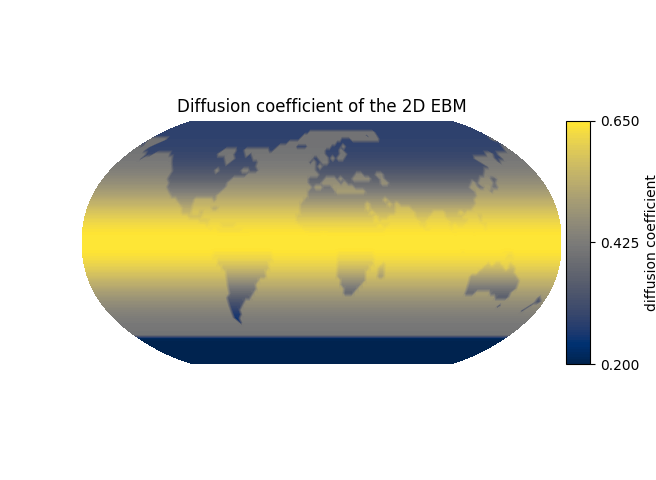
\includegraphics[width=0.6\linewidth,center]{figs/diffusion_coefficients.png}
\caption{Diffusion coefficients}
\end{figure}

\begin{figure}[!htb]
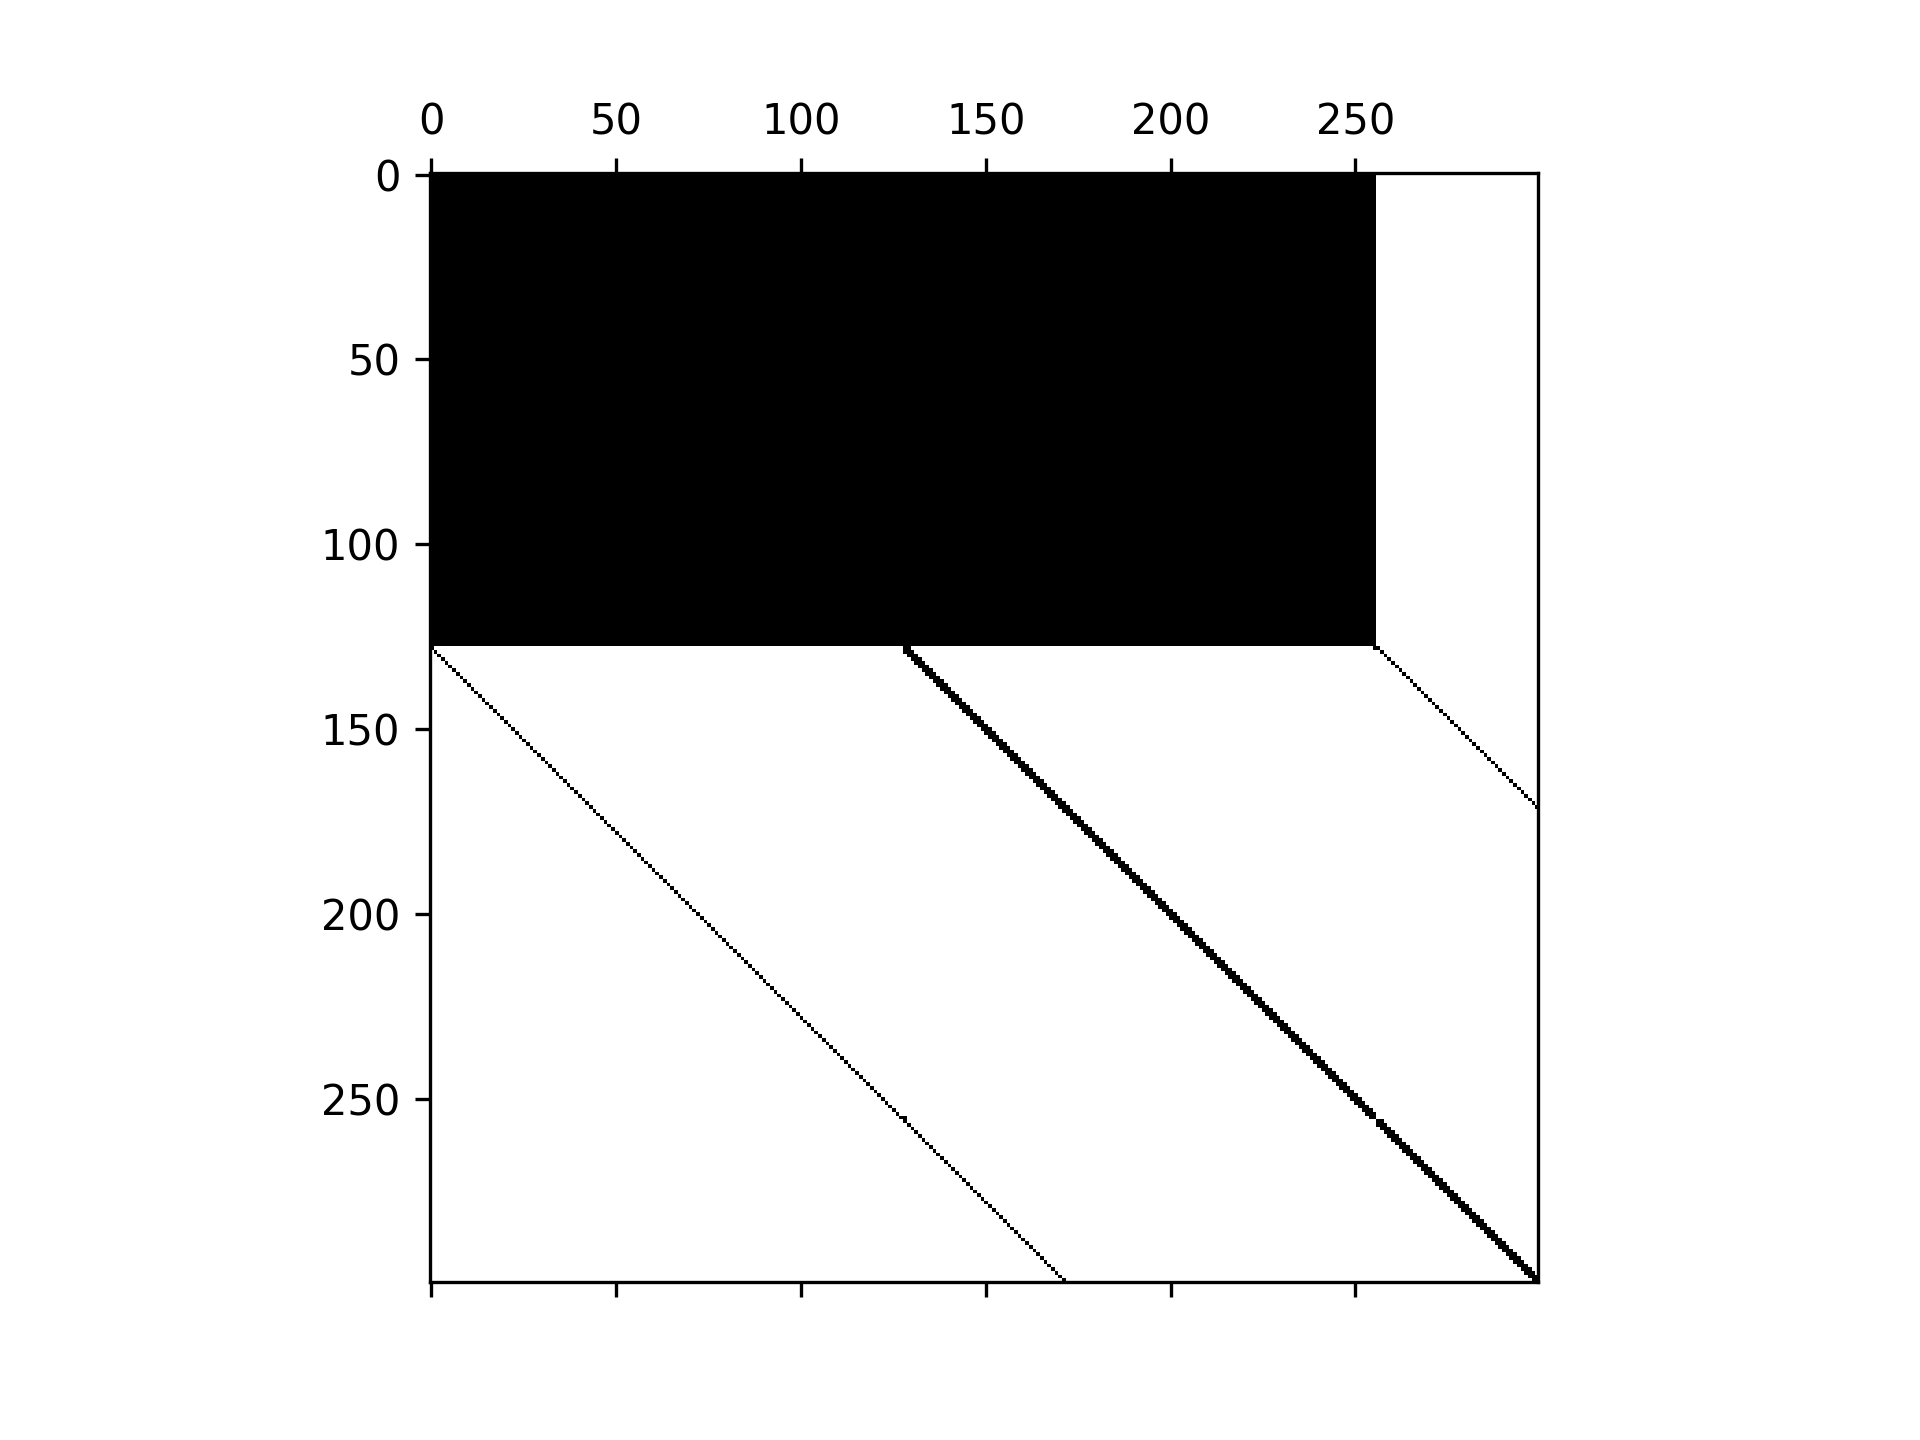
\includegraphics[width=0.6\linewidth,center]{figs/sparsity_pattern.png}
\caption{Sparsity pattern of the upper left part of the system matrix}
\end{figure}


\end{document}
